\clearpage
\hypertarget{conBran vis}{}
\subsection{Visual; (original)}
\visHeader

Perform the following steps to branch with a \texttt{StatementNode}:
\begin{enumerate}
\item[$\blacktriangleright$] Add a new statement node (cf.~Fig.~\ref{fig:cond_statement_node}) at the appropriate location in your SDM.
\item[$\blacktriangleright$] Invoke a non-void method (an operation in the metamodel) via a \texttt{MethodCallExpression} (cf.~Fig.~\ref{fig:cond_method_call}).
\item[$\blacktriangleright$] Add \texttt{Success} \emph{and} \texttt{Failure} edges to the \texttt{StatementNode} to branch appropriately.
\end{enumerate}

\begin{figure}[htp]
\begin{center}
  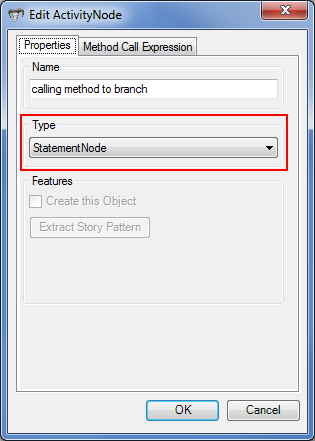
\includegraphics[width=0.5\textwidth]{01_switch_to_statement_node}
  \caption{Switch from activity node to statement node}
  \label{fig:cond_statement_node}
\end{center}
\end{figure}

\begin{figure}[htp]
\begin{center}
  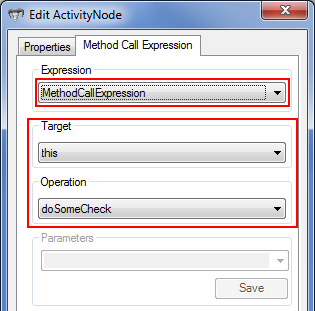
\includegraphics[width=0.5\textwidth]{02_specify_method_call_expression}
  \caption{Specify the method call expression}
  \label{fig:cond_method_call}
\end{center}
\end{figure}

Fig.~\ref{fig:cond_branch_on_op_code} depicts the corresponding generated if/else branch in Java.

\begin{figure}[htp]
\begin{center}
  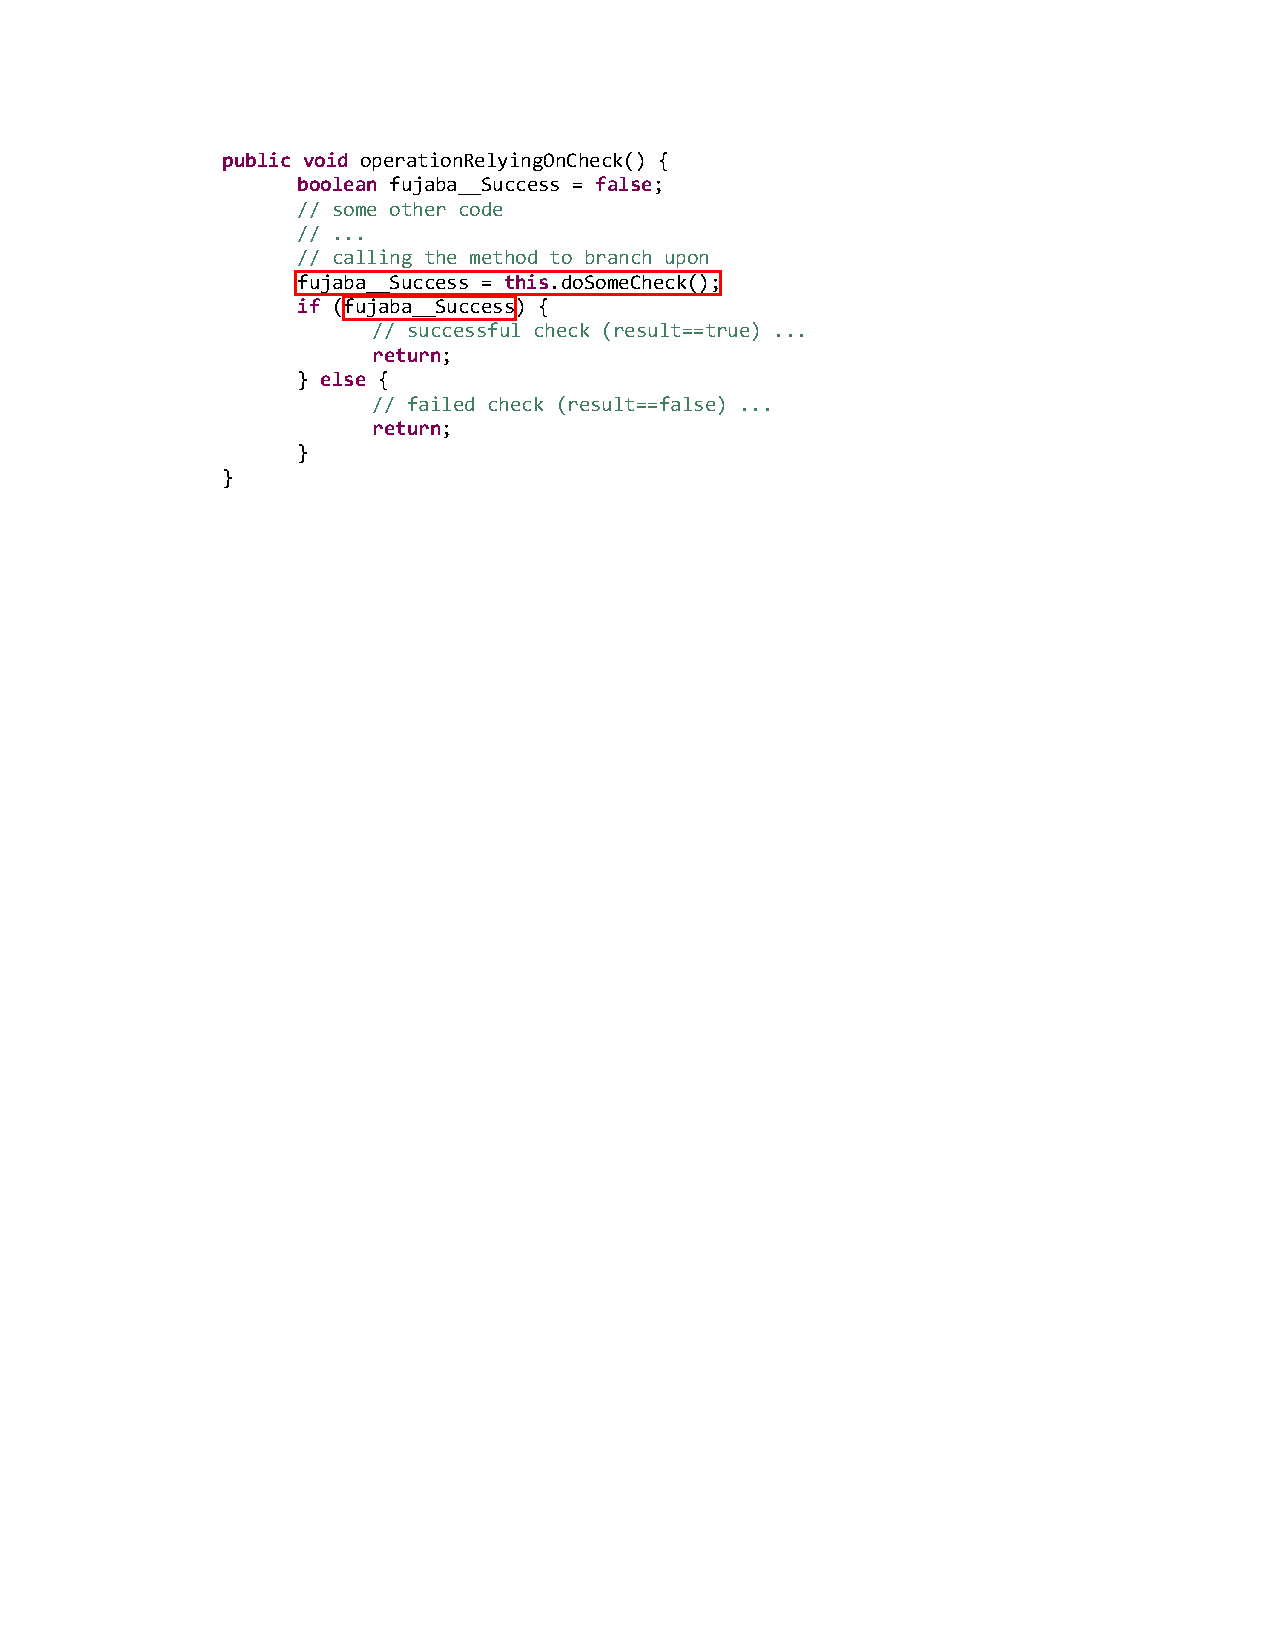
\includegraphics[width=0.7\textwidth]{generated_code}
  \caption{Generated code for branch}
  \label{fig:cond_branch_on_op_code}
\end{center}
\end{figure}
